\documentclass[a4paper,12pt]{report}
\usepackage{myStyle}

% Acronyms

\newacronym{EEG}{EEG}{electroencephalography}
\newacronym{BCI}{BCI}{brain-computer interface}
\newacronym{FFT}{FFT}{fast Fourier transform}
\newacronym{CCA}{CCA}{canonical correlation analysis}
\newacronym{MEG}{MEG}{magnetoencephalography}
\newacronym{fMRI}{fMRI}{functional magnetic resonance imaging}
\newacronym{PET}{PET}{positron emission tomography}
\newacronym{fNIRS}{fNIRS}{functional near-infrared spectroscopy}
\newacronym{ERP}{ERP}{event-related potential}
\newacronym{VEP}{VEP}{visual evoked potential}
\newacronym{SSVEP}{SSVEP}{steady-state visual evoked potential}
\newacronym{ADC}{ADC}{analog-to-digital converter}
\newacronym{SC}{SC}{stability coefficient}
\newacronym{PSDA}{PSDA}{power spectrum density analysis}
\newacronym{MEC}{MEC}{minimum energy combination}
\newacronym{LASSO}{LASSO}{least absolute shrinkage and selection operator}
\newacronym{LRT}{LRT}{likelihood ratio test}
\newacronym{MPCC}{MCPP}{multi-phase cycle coding}

\newglossaryentry{neuron}{
	name = neuron,
	description = {-- nerve cell}
}
\newglossaryentry{dendrite}{
	name = dendrite,
	description = {-- nerve ending}
}
\newglossaryentry{axon}{
	name = axon,
	description = {-- nerve fibre}
}
\newglossaryentry{synapse}{
	name = synapse,
	description = {-- connection between neurons}
}
\newglossaryentry{neural pathway}{
	name = neural pathway,
	description = {-- network formed by functionally related neurons}
}
\newglossaryentry{membrane potential}{
	name = membrane potential,
	description = {-- difference between the interior and the exterior of a cell}
}
\newglossaryentry{resting state}{
	name = resting state,
	description = {-- the state of a neuron that is not exited and not sending signals at the moment}
}
\newglossaryentry{resting potential}{
	name = resting potential,
	description = {-- the membrane potential of a neuron at a resting state}
}
\newglossaryentry{action potential}{
	name = action potential,
	description = {-- the event of sending signals used by neurons}
}
\newglossaryentry{ionophoric protein}{
	name = ionophoric protein,
	description = {-- proteins used to transport ions across cell membrane}
}
\newglossaryentry{threshold potential}{
	name = threshold potential,
	description = {-- certain threshold value. If membrane potential exceeds threshold potential, action potential is initiated}
}
\newglossaryentry{postsynaptic cell}{
	name = postsynaptic cell,
	description = {-- a cell that received a signal through synapse. This term is used for example when discussing single action potential and its effect on the cell that receives the signal}
}
\newglossaryentry{postsynaptic potential}{
	name = postsynaptic potential,
	description = {-- change in the membrane potential in a postsynaptic cell caused by synaptic input}
}
\newglossaryentry{sink}{
	name = sink,
	description = {-- location where ions enter the postsynaptic cell after synaptic input has been received}
}
\newglossaryentry{source}{
	name = source,
	description = {-- location where ions exit the postsynaptic cell after synaptic input has been received to achieve electroneutrality}
}
\newglossaryentry{dipole}{
	name = dipole,
	description = {-- formed by a sink and a source around postsynaptic cell. Dipoles produce electric field that can be measured from the scalp using EEG.}
}

% Packages for layout testing

%\usepackage{showframe}
%\usepackage{layouts}
%\usepackage{layout}
%\printinunitsof{pt}

\includeonly{./tex/abstract, ./tex/title_page, ./tex/appendices, ./tex/introduction, ./tex/EEG, ./tex/BCI, ./tex/conclusion, ./tex/SSVEP_BCI, ./tex/results}
\begin{document}

%\layout
%\pagevalues
%\newpage

% Title page
% font size table: http://tex.stackexchange.com/questions/24599/what-point-pt-font-size-are-large-etc

\begin{center}
\thispagestyle{empty}
\large{UNIVERSITY OF TARTU}\\
\large{FACULTY OF MATHEMATICS AND COMPUTER SCIENCE}\\
\large{Institute of Computer Science}\\
\large{Computer Science Curriculum}\\
\vspace{160pt}
\Large{\bf Anti Ingel}\\
\vspace{6pt}
\LARGE{\textbf{Control a Robot via VEP Using \\Emotiv EPOC}}\\
\vspace{12pt}
\large{\bf Bachelor's Thesis (9 ECTS)}
\vspace{63pt}
\end{center}
\hfill \Large{Supervisor: Ilya Kuzovkin}
\vfill
\begin{center}
\large{Tartu 2015}
\end{center}

\selectlanguage{english}
\chapter*{Control a Robot via VEP Using Emotiv EPOC}

\section*{Abstract}

\normalsize
This thesis describes an \acrshort{SSVEP}-based \acrshort{BCI} implemented as a practical part of this thesis. One possible usage of a \acrshort{BCI} that efficiently implements a communication channel between the brain and an external device would help severely disabled people to control devices that currently require pushing buttons, for example an electric wheelchair. The \acrshort{BCI} implemented as a part of this thesis uses widely known \acrshort{PSDA} and \acrshort{CCA} feature extraction methods and introduces a new way to combine these methods. Combining different methods improves the performance of a \acrshort{BCI}. The \acrshort{BCI} is open-source, written in Python 2.7, has graphical user interface and uses inexpensive \acrshort{EEG} device called Emotiv EPOC. The \acrshort{BCI} requires only a computer and Emotiv EPOC, no additional hardware is needed. Different \acrshort{EEG} devices could be used after modifying the code. 

\section*{Keywords}

\acrshort{EEG}, electroencephalography, \acrshort{BCI}, brain-computer interface, f-VEP, frequency-modulated visual evoked potential, \acrshort{SSVEP}, steady-state visual evoked potential, \acrshort{CCA}, canonical correlation analysis, \acrshort{PSDA}, power spectral density analysis, open-source
\selectlanguage{estonian}
\chapter*{Visuaalse stiimuliga esilekutsutud potentsiaalidel põhinev roboti juhtimine Emotiv EPOC seadmega}

\section*{Lühikokkuvõte}

Antud töö kirjeldab visuaalse stiimuliga esilekutsutud potentsiaalidel põhinevat aju ning arvuti vahelist liidest (AAL), mis loodi antud töö praktilise osana. AALi saab kasutada aju ja seadme vahelise otsese suhtluskanali loomiseks, mis tähendab, et seadmega suhtlemiseks pole vaja nuppe vajutada, piisab vaid visuaalsete stiimulite vaatamisest. Efektiivne AAL võimaldaks raske puudega isikutel näiteks elektroonilist ratastooli juhtida. Antud töö osana loodud AAL kasutab tuntud kanoonilise korrelatsiooni- ja võimsusspektri analüüsi meetodeid ning uuendusena kombineerib need kaks meetodit üheks teineteist täiendavaks meetodiks. Kahe meetodi kombinatsioon muudab AALi täpsemaks. Antud AAL on avatud lähtekoodiga, kirjutatud Python 2.7 programmeerimiskeeles, sisaldab graafilist kasutajaliidest ning kasutab aju tegevuse mõõtmiseks elektroensefalograafia (EEG) seadet Emotiv EPOC. AALi kasutamiseks on vaja ainult arvutit ja Emotiv EPOC seadet. Koodi muutes on võimalik kasutada ka teisi EEG seadmeid. 

\section*{Võtmesõnad}

EEG, elektroensefalograafia, AAL, aju-arvuti liides, visuaalne stiimul, kanooniline korrelatisoonianalüüs, võimsusspektri analüüs, avatud lähtekood
\selectlanguage{english}

\tableofcontents
\addcontentsline{toc}{chapter}{Introduction}

\chapter*{Introduction}

Over the last decade the question how to implement direct communication channel between the brain and an external device has received much attention~\cite{mec, cca_lin, MPCC, sc, LRT, LASSO}. This communication channel works by translating recorded brain activity into commands to control the device or the other way round---by sending signals into the brain. Sending signals into the brain requires a surgery to implant the device that can send those signals. This approach can be used for example to repair damaged vision or hearing.

Measuring the brain activity, however, can be done without implanting devices into the brain and therefore it is easier and less expensive than invasive methods. This approach can be used for example to operate a wheelchair or for typing without having to press buttons. Nowadays the brain activity can be measured using non-invasive and inexpensive devices and thus many people could benefit from an application that efficiently implements this new communication channel between the brain and an external device.

This thesis describes an application that uses an \gls{EEG} device called Emotiv EPOC to measure brain activity and translates the recorded signal into commands to control a robot. The application was written as a practical part of this thesis and the focus was on implementing an inexpensive application. Compared to existing applications, the practical part of this thesis combines two widely used methods called \gls{PSDA}~\cite{psda} and \gls{CCA}~\cite{cca_lin} for extracting information from brain recording in a way which to the best of the author's knowledge has not been done before.

The first chapter of this thesis describes the biology of the brain and discusses, what aspect of the brain activity can actually be measured. In this chapter also different techniques and devices that can be used to measure brain activity are compared.

The second chapter describes how to evoke a brain response that can be extracted from the recording of brain activity using only Emotiv EPOC and a laptop computer. The methods that can be used to analyse the recording are discussed in this chapter.

The third chapter describes the application implemented as a practical part of this thesis. This chapter contains overview of related works, describes the signal processing and explains the novelty of the application.


\chapter{Electrical activity in the brain}

The aim of this chapter is to describe the biology of the brain, discuss how brain activity can be measured and where the measurable activity originates from. The chapter will also compare different techniques and devices used to measure brain activity and finally suitable device for controlling a robot is chosen.

\section{Source of the electrical activity}
\label{sec:neuron}

As all living organisms are composed of cells, so are humans and the human brain. The brain consists of nerve cells called \glspl{neuron} and non-neural cells. There are approximately 86 billion \glspl{neuron} in the human brain and roughly as much non-neural cells~\cite{neuroncount}. The aim of this section is to describe how \glspl{neuron} interact with each other and discuss what aspect of this communication can be measured.

\begin{figure}[b!]
	\centering
	\begin{subfigure}{0.48\textwidth}
		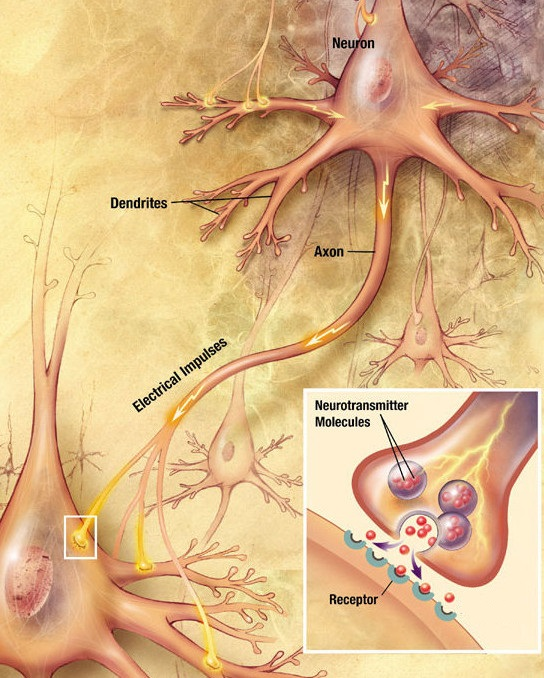
\includegraphics[width=\textwidth]{synapse_modified.jpg}
		\caption{Neurons and a chemical synapse~\cite[p.~17]{neuronpic}}
		\label{fig:neuron_synapse}
	\end{subfigure}
	~
	\begin{subfigure}{0.48\textwidth}
		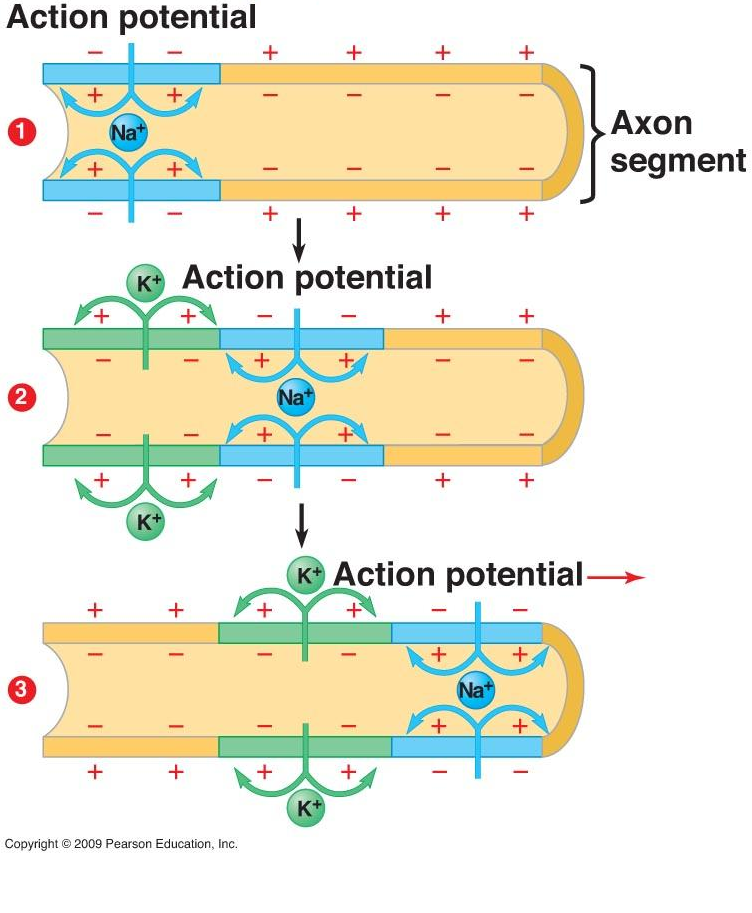
\includegraphics[width=\textwidth]{action_potential.png}
		\caption{Action potential~\cite{action_potential_pic}}
		\label{fig:action_potential}
	\end{subfigure}
	\caption{The structure of a neuron}
\end{figure}

A typical \gls{neuron} has a cell body, multiple nerve endings or \glspl{dendrite}, and one nerve fibre or \gls{axon}. Both \glspl{dendrite} and \glspl{axon} can branch multiple times. \Glspl{neuron} interact with each other via electro-chemical signals that are transmitted through various connections. These connections are not static and can change over time. The connection between an \gls{axon} and a \gls{dendrite} is called a \gls{synapse}. See figure~\ref{fig:neuron_synapse} for an example of \glspl{neuron} and a \gls{synapse}. The general rule is that a \gls{neuron} sends signals through its \gls{axon} and receives signals through \glspl{dendrite}. Functionally related \glspl{neuron} are connected to each other and form \glspl{neural pathway}~\cite{neuralpathway}.

To send signals, \glspl{neuron} must be able to maintain electric potential called \gls{membrane potential}. \Gls{membrane potential} is the difference in electric potential between the interior and the exterior of a cell. When a \gls{neuron} is not sending signals or in other words, when neuron is at a \gls{resting state}, its \gls{membrane potential} is slightly negative. The \gls{membrane potential} of a \gls{neuron} at a \gls{resting state} is called \gls{resting potential}. Negative \gls{resting potential} is achieved by having more positively charged ions around the cell than inside the cell.

By having stable \gls{resting potential}, \glspl{neuron} are able to send signals by rapidly increasing and decreasing the \gls{membrane potential} along an \gls{axon}. This event is called an \gls{action potential}. See figure~\ref{fig:action_potential} for example. To increase or decrease the \gls{membrane potential} of a cell, \glspl{ionophoric protein} are used. These proteins transport ions across the cell membrane to regulate the concentration of ions inside the cell. Since ions are electrically charged, the concentration of ions inside a cell affects the \gls{membrane potential} of the cell. The \gls{membrane potential} of a cell can be increased by transporting positive ions into the cell and decreased by transporting positive ions out of the cell. 

An \gls{action potential} or signal sending is initiated when the \gls{membrane potential} of a \gls{neuron} exceeds certain threshold value called \gls{threshold potential}. The \gls{membrane potential} of a \gls{neuron} can increase when the \gls{neuron} receives signals from other \glspl{neuron}. The \gls{neuron} that receives a signal is called \gls{postsynaptic cell}. The received signal can cause the \gls{membrane potential} of the \gls{postsynaptic cell} to increase or decrease. This change in \gls{membrane potential} is called a \gls{postsynaptic potential}. If the \gls{postsynaptic potential} is large enough for the \gls{membrane potential} to exceed \gls{threshold potential}, an \gls{action potential} is initiated in the \gls{postsynaptic cell}.

The following paragraph is mainly based on the article by Buzsaki \textit{et al.}~\cite{electric_field}. The \gls{postsynaptic potential} is caused by ions flowing into the cell. To achieve electroneutrality, a balancing flow of ions from the interior to the exterior of the cell is needed. The ions of the balancing flow have the same electric charge as the entering ions. If the ions flowing into the cell have
\begin{itemize}
	\item positive charge, then 
	\subitem the \gls{membrane potential} of the cell increases,
	\subitem location where positive ions enter the cell is called a \gls{sink},
	\subitem location where positive ions exit the cell is called a \gls{source} and
	\subitem positive ions are gathered from the \gls{sink} and accumulated around the \gls{source}.
	\item negative charge, then
	\subitem the \gls{membrane potential} of the cell decreases,
	\subitem location where negative ions enter the cell is called a \gls{source},
	\subitem location where negative ions exit the cell is called a \gls{sink} and
	\subitem negative ions are gathered from the \gls{source} and accumulated around the \gls{sink}.
\end{itemize}

In both cases, the \gls{source} has more positive electrical charge than the \gls{sink}. Since the \gls{source} and the \gls{sink} have different electric potentials, they form a \gls{dipole}. See figure~\ref{fig:dipole} for illustration.

\begin{figure}[h!]
	\centering
	\begin{subfigure}{0.48\textwidth}
		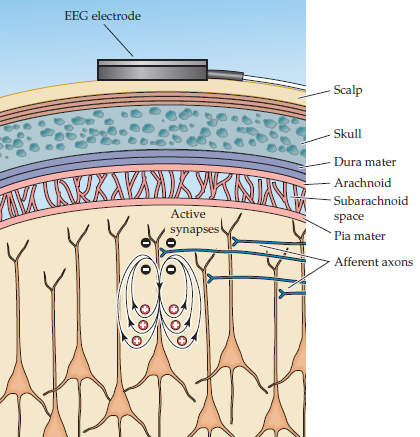
\includegraphics[width=\textwidth]{dipole_neuron.png}
		\caption{Dipole generated by a neuron~\cite[p.~669]{neuroscience}}
		\label{fig:dipole_neuron}
	\end{subfigure}
	~
	\begin{subfigure}{0.48\textwidth}
		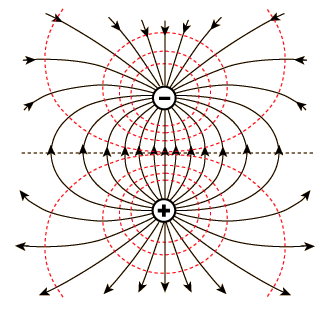
\includegraphics[width=\textwidth]{dipole_electric.png}
		\caption{The electric field of a dipole\protect\footnotemark}
		\label{fig:dipole_electric}
	\end{subfigure}
	\caption{Dipoles}
	\label{fig:dipole}
\end{figure}
\footnotetext{http://hyperphysics.phy-astr.gsu.edu/hbase/electric/equipot.html}

These \glspl{dipole} are important because it is possible to measure the electric field produced by these \glspl{dipole} from the scalp. See figure~\ref{fig:dipole_neuron} for illustration. Measuring these electric fields is further discussed in section~\ref{sec:EEG}. Although \glspl{action potential} generate stronger currents than \glspl{postsynaptic potential}, their duration is short and nearby \glspl{neuron} rarely fire synchronously~\cite{electric_field}. Thus recording the electrical activity of the brain mainly relies on the electric fields of the \glspl{dipole} generated by \glspl{neuron}.

\section{Functional neuroimaging methods}
\label{sec:neuroimaging}

As discussed in section~\ref{sec:neuron}, \glspl{neuron} in the brain are sending electrochemical signals to communicate with each other. There are several techniques available to measure this activity. The aim of this section is to briefly compare various non-invasive techniques. Measuring an aspect of brain function is called \gls{functional neuroimaging} and common measurement methods divide into \gls{haemodynamic} and \gls{electromagnetic} techniques.

\Gls{haemodynamic} techniques measure blood oxygenation and blood flow in the brain. More oxygen has to be delivered to more active brain regions and this allows the brain activity to be measured. \Gls{haemodynamic} techniques include \gls{fMRI}, \gls{fNIRS} and \gls{PET}.

\Gls{electromagnetic} techniques measure either electrical activity or magnetic fields produced by the electrical activity along the scalp. \Gls{electromagnetic} techniques include \gls{EEG} and \gls{MEG}. These methods have lower \gls{temporal resolution} than \gls{haemodynamic} methods, but measure only the activity in the outer layer of the brain. \Gls{temporal resolution} is the smallest time period of neural activity that is reliably separated out by measuring technique.

To decide which method is best for controlling a robot, cost, portability and \gls{temporal resolution} of each method is compared. See table~\ref{tab:neuroimaging} for details. For real-time robot controlling, lower \gls{temporal resolution} is better because it enables faster decision making.

% Constants for table

\newcommand{\pMEG}{\tablefootnote{http://neurogadget.com/2012/12/15/inexpensive-magnetoencephalography-meg-system-could-be-available-at-every-hospital/6495}}
\newcommand{\pfMRI}{\tablefootnote{http://info.blockimaging.com/bid/92623/MRI-Machine-Cost-and-Price-Guide}}
\newcommand{\pPET}{\tablefootnote{http://info.blockimaging.com/bid/68875/How-Much-Does-a-PET-CT-Scanner-Cost}}
\newcommand{\pEEG}{\tablefootnote{http://en.wikipedia.org/wiki/Comparison\_of\_consumer\_brain-computer\_interfaces}}
\newcommand{\pNIRS}{\cite{NIRS}}
\newcommand{\tresol}{\cite{timeresol}}

% Table

\begin{table}[h]
	\centering
	\begin{tabular}{|c|c|c|c|c|c|}\hline
			& Price	from				& Portable	& Temporal resolution		& Special requirements			\\\hline
\gls{MEG}	& millions\pMEG				& no		& milliseconds~\tresol		& magnetically shielded room	\\\hline
\gls{fMRI}	& \SI{150000}[\$]\pfMRI		& no		& about 1 second~\tresol	& magnetically shielded room	\\\hline
\gls{PET}	& \SI{125000}[\$]\pPET		& no		& about 1 second~\tresol	& radioactive isotopes injection\\\hline
\gls{fNIRS}	& \SI{10000}[\$]{}~\pNIRS	& yes		& over 0.1 second~\pNIRS	&								\\\hline
\gls{EEG}	& \SI{45}[\$]\pEEG			& yes		& milliseconds~\tresol		&								\\\hline
	\end{tabular}
	\caption{Comparison of functional neuroimaging methods}
	\label{tab:neuroimaging}
\end{table}

In this thesis, techniques that are portable and available to the consumer are preferred, so the usage would not be limited to certain location and would be available to the people in need. Considering all these arguments, it can be seen that currently the best choice for controlling a robot is an \gls{EEG} device.

\section{Electroencephalography}
\label{sec:EEG}

As already mentioned in the previous section, \gls{EEG} measures the electrical activity along the scalp. This electrical activity originates mainly from the electric fields generated by \glspl{neuron} as discussed in section~\ref{sec:neuron}. The aim of this section is to describe the basics of \gls{EEG} and discuss how brain activity evoked by certain event can be measured using \gls{EEG}.

The electric potential generated by one \gls{neuron} is far too low to be recognized. Therefore, approximately 108 \glspl{neuron} have to have synchronous electrical activity to a create measurable field~\cite{field_count}. Furthermore, these \glspl{neuron} have to have certain orientation for the electric fields to add up and reach the electrode on the scalp. Namely, these neurons need to be perpendicular to the surface of the brain. See figure~\ref{fig:dipole_neuron} for example.

\gls{EEG} measures the potential fields as the function of voltage versus time using electrodes placed on scalp~\cite{field_count}. Since voltage is the electric potential difference between two points, one or more reference electrodes are commonly used. Then voltmeter can be used to measure the differences in voltage between two electrodes, one of which is the reference electrode. See figure~\ref{fig:voltmeter} for a simplified scheme.

\begin{figure}[h!]
	\centering
	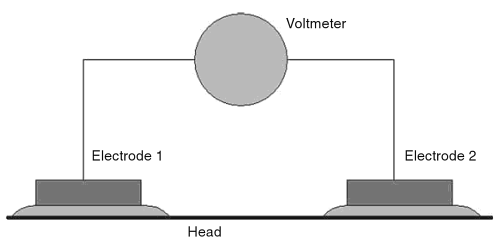
\includegraphics[width=0.70\textwidth]{voltmeter.png}
	\caption{Electrodes connected to a voltmeter~\cite[p.~120]{ERP}}
	\label{fig:voltmeter}
\end{figure}

Usually electrodes are placed on the scalp according to international 10-20 electrode location system. The outer layer of the brain can be classified into four lobes: temporal, occipital, parietal and frontal. See figure~\ref{fig:brain_lobes} for example. 10-20 electrode location system uses a letter and a number to identify electrode location. The letter is the first letter of the brain lobe above which the electrode is located and therefore the electrode measures the activity of this brain lobe. There are more complicated electrode-naming-systems that extend the 10-20 system. See figure~\ref{fig:electrode_locations} for illustration.

In a broad sense, \gls{EEG} recording is linked to the general state of the brain~\cite{VEP}. Therefore, due to the generality of the recording, potentials evoked by certain events cannot be seen in the recording because the evoked potentials are much smaller than the general fluctuations. A brain potential evoked by some event is called \gls{ERP}. 

\glspl{ERP} are linked to the information flow in the brain and are usually recorded by using an averaging technique~\cite{ERP}. For example, \glspl{ERP} can be recorded by presenting a stimulus with a certain time interval to a subject and calculating the average of \gls{EEG} signals recorded in the same time interval. This technique can be used because the stimuli is presented at a constant rate and thus \glspl{ERP} are also evoked one after another in the same constant interval. Therefore, \glspl{ERP} are always evoked at the same time while other fluctuations and noise are mostly random. When calculating the average of the \gls{EEG} recordings divided into the same time intervals as the stimulus presentation, the result will be an \gls{ERP} because other fluctuations and noise mostly cancel out in the averaging process. Thus \gls{EEG} can be used to record \glspl{ERP} from the scalp. 

\section{Visual evoked potential}
\label{sec:VEP}

In section~\ref{sec:EEG} brain potential called \gls{ERP} was discussed and it was noted that \glspl{ERP} are evoked by some event. The aim of this section is to discuss one specific \gls{ERP} called \gls{VEP}. As the name suggests, \glspl{VEP} are elicited by visual stimuli. The visual stimulus for eliciting a \gls{VEP} can be very simple, for example a white square blinking on a black computer screen.

When the visual stimulus is seen, the signal travels from the eyes to the \gls{visual processing centre} through the \gls{primary visual pathway}~\cite{neuroscience}. The \gls{visual processing centre} is located in the back of the brain. As mentioned in section~\ref{sec:EEG}, the outer layer of the brain can be classified into four lobes. The \gls{visual processing centre} is located in the occipital lobe. See figure~\ref{fig:lobes_pathway} for illustration. The \gls{primary visual pathway} is a \gls{neural pathway}; \glspl{neural pathway} were also mentioned in the section~\ref{sec:neuron}.

\begin{figure}[h]
	\centering
	\begin{subfigure}{0.48\textwidth}
		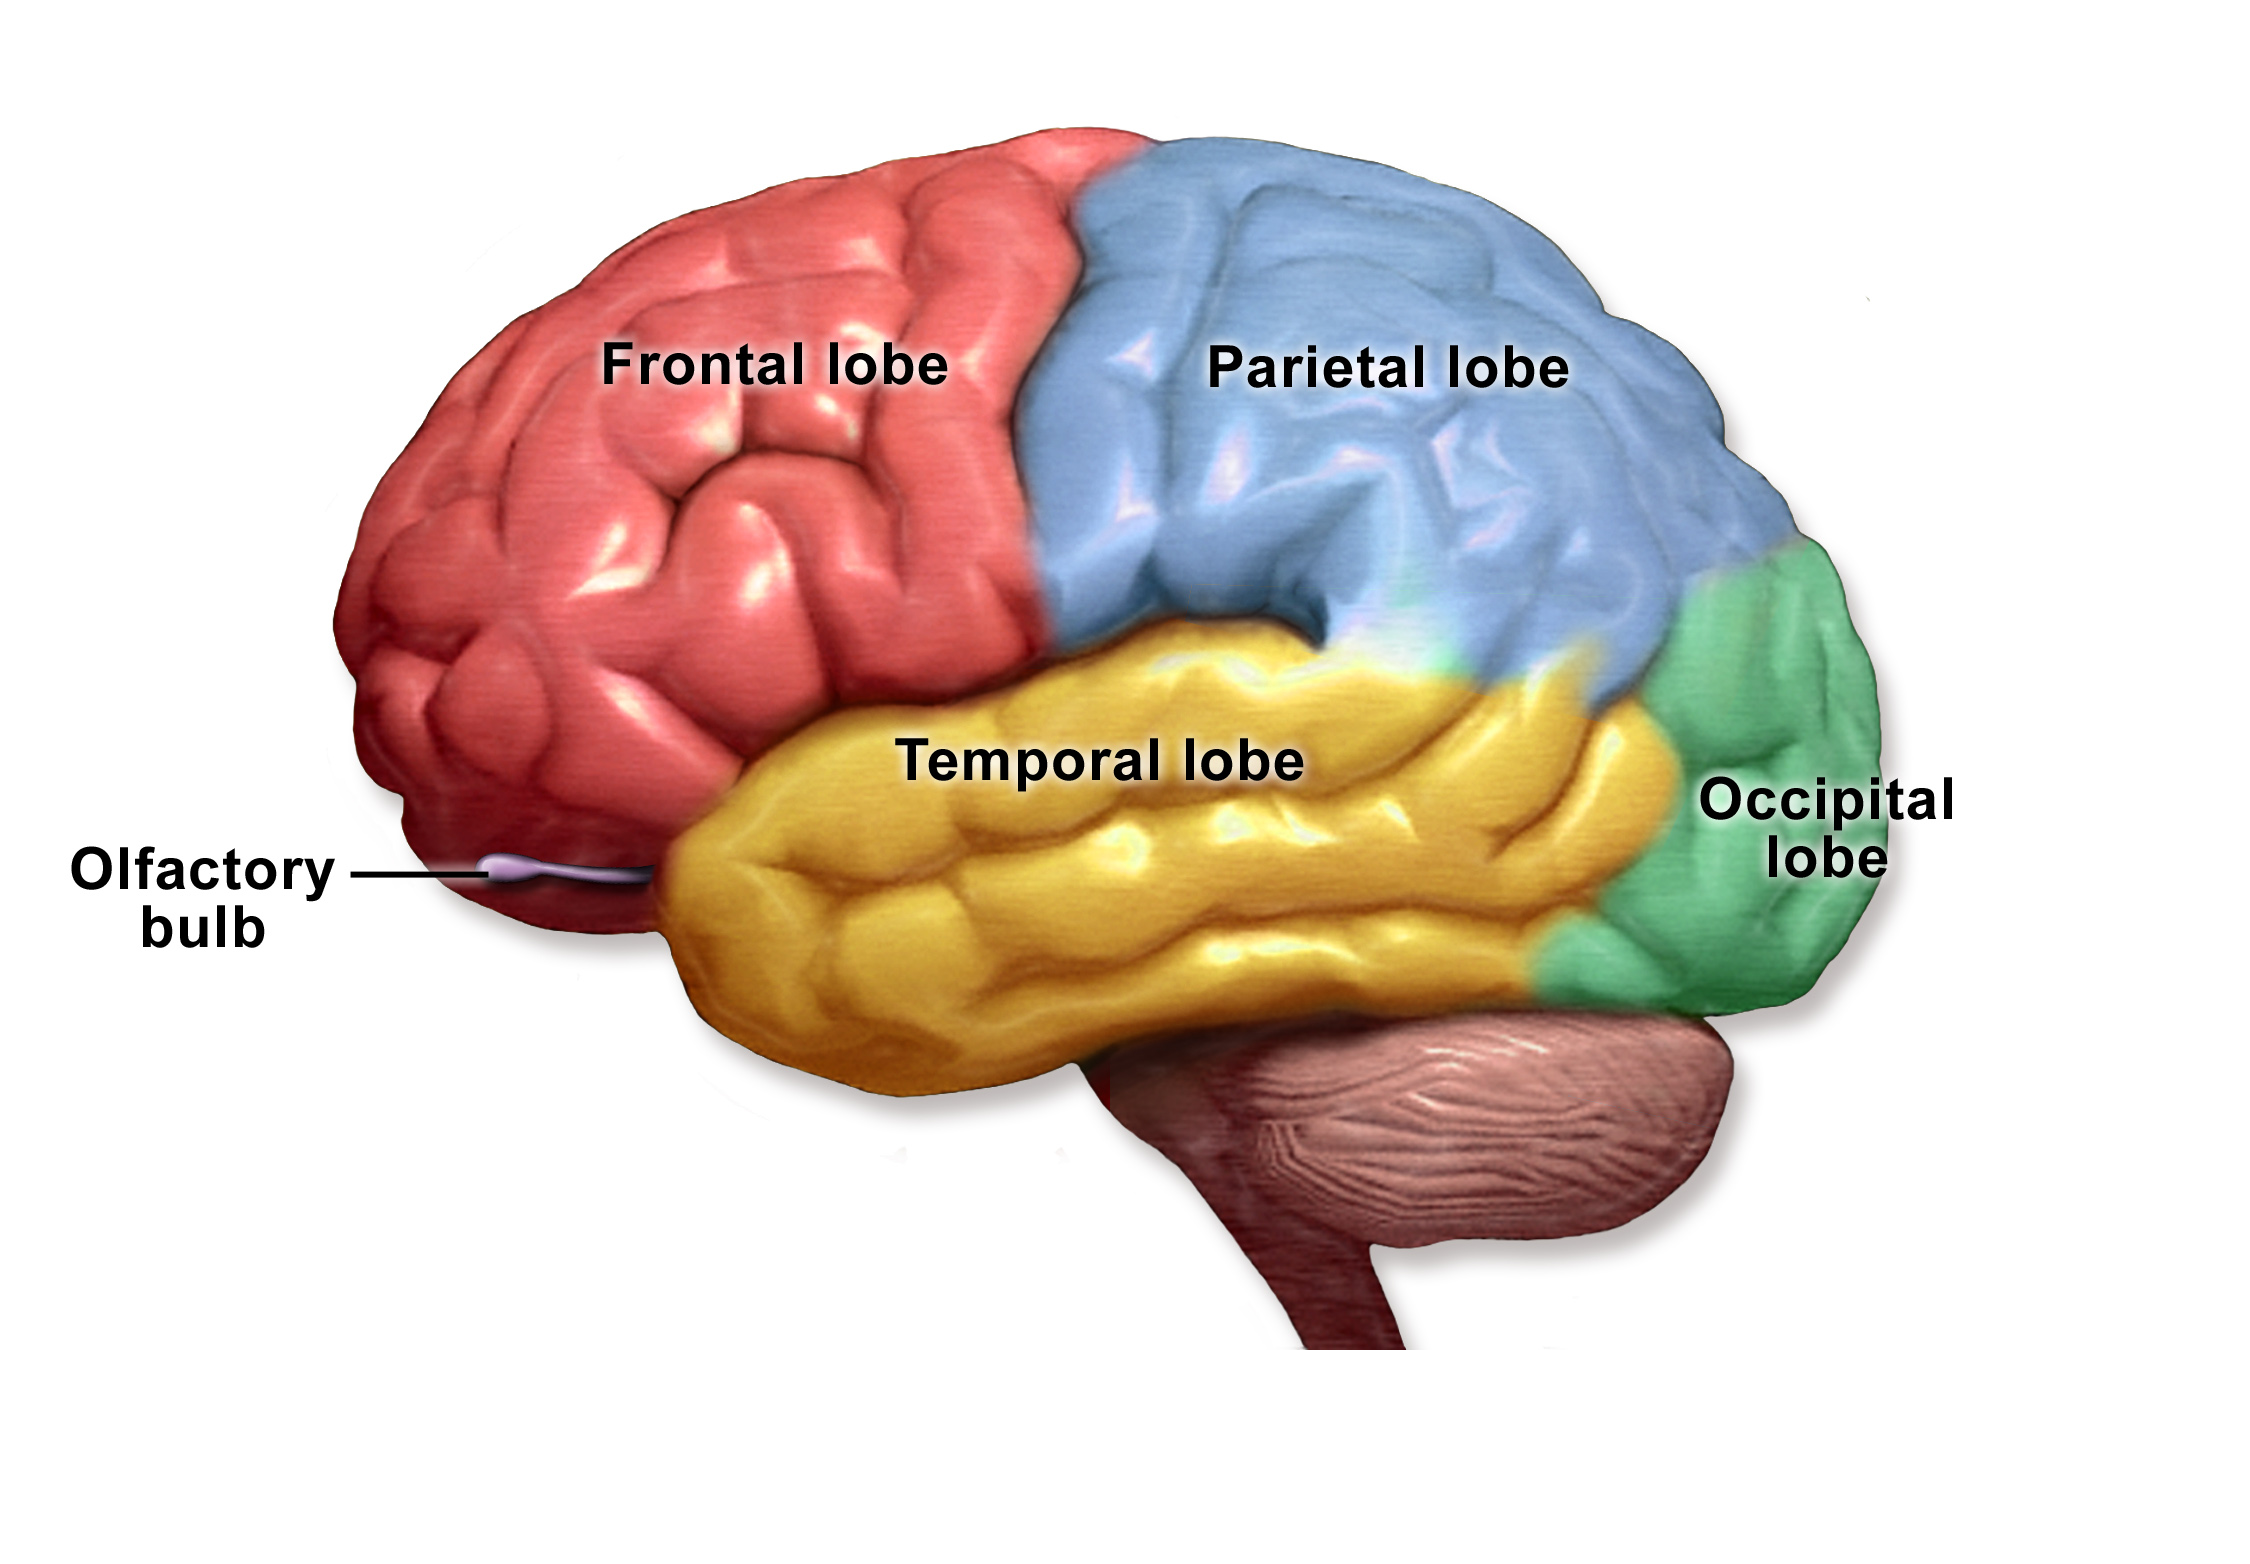
\includegraphics[width=\textwidth]{brain_lobes.png}
		\caption{Lobes of the brain~\cite{blausen}}
		\label{fig:brain_lobes}
	\end{subfigure}
	~
	\begin{subfigure}{0.48\textwidth}
		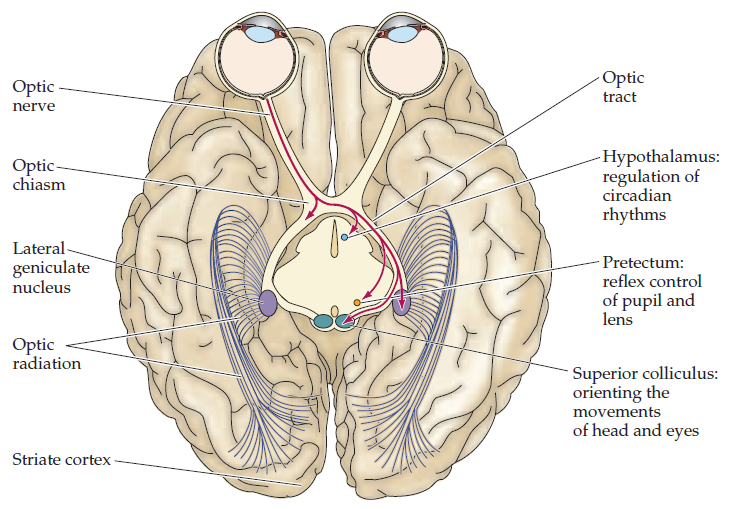
\includegraphics[width=\textwidth]{visual_pathway.png}
		\caption{The primary visual pathway~\cite[p.~261]{neuroscience}}
		\label{fig:visual_pathway}
	\end{subfigure}
	\caption{The location of occipital lobe and the neural pathway from eyes to the lobe}
	\label{fig:lobes_pathway}
\end{figure}

Due to the posterior location of the occipital lobe, electrodes must be placed to the back of the head when recording \glspl{VEP} with \gls{EEG}. These electrode locations are identified with the letter O as discussed in section~\ref{sec:EEG}.

When comparing the \glspl{VEP} elicited by
\begin{enumerate*}[(1)]
	\item the stimulation of the \gls{central visual field} and
	\item the stimulation of the \gls{peripheral vision}
\end{enumerate*} by the same stimuli, it can be seen that the stimulation of the \gls{central visual field} produces larger \glspl{VEP}~\cite{VEP_size}. In other words, the stimulus which a subject is looking at elicits larger \glspl{VEP} than those stimuli that are not in the very centre of gaze. Therefore, it is possible to present multiple visual stimuli to a subject and detect which stimulus is the subject looking at. 

To make the detection of \glspl{VEP} easier, \glspl{SSVEP} are used. If the visual stimulus is presented at a constant rate and the rate is so fast that the visual pathway does not have enough time to fully recover between stimulus presentations, then the elicited response becomes continuous and it is called the \gls{SSVEP}~\cite{VEP}. See figure X for an example of \gls{VEP} and \gls{SSVEP}. \gls{SSVEP} is continuous and therefore it is easier to detect it in \gls{EEG} recording than \glspl{VEP}, which are not continuous. Detecting continuous response is easier because it is always present in the recording. The methods used to detect \gls{SSVEP} in \gls{EEG} recording are discussed in section~\ref{sec:SSVEP_detection}.

Research has shown that \glspl{SSVEP} reflect certain properties of the visual stimulus. The \gls{SSVEP} is composed of components that have different frequencies. The visual stimuli and signal components are further discussed in section~\ref{sec:stimuli} and section~\ref{sec:fourier} respectively. The frequency of the component that has the highest amplitude is the same as the \gls{fundamental frequency} or the lowest frequency of the visual stimulus. Thus \gls{SSVEP} can be detected in \gls{EEG} recording by finding and analysing the components of \gls{SSVEP} in the recording.
%The frequency of \gls{SSVEP} elicited by a visual stimulus is the same as the presentation rate or \gls{flickering} frequency of the visual stimulus. Furthermore, not only the frequency of the visual stimulus can be detected in the \gls{EEG} recording, but also its \glspl{harmonic}. \Glspl{harmonic} are components of \gls{SSVEP} that have frequency which is integer multiple of the fundamental frequency. Thus \gls{SSVEP} is composed of components each of which has frequency that is integer multiple of the lowest frequency in \gls{SSVEP}.

\section{Emotiv EPOC}
\label{sec:EEG_comparison}

In section~\ref{sec:neuroimaging} different functional neuroimaging methods were compared and it was concluded that currently \gls{EEG} is most suitable for designing inexpensive and portable interface for controlling a robot. But there is a wide variety of EEG devices available. The aim of this section is to briefly compare some of the devices and choose inexpensive and portable device available to the consumer.

Continuous signal cannot be directly represented in computers or in other digital devices and therefore continuous signal has to be converted to discrete signal to process it with a computer. As already mentioned in section~\ref{sec:EEG}, \gls{EEG} measures brain activity as function of voltage versus time. This function represents discrete signal, which means that both voltage and time are discrete. In other words, there is a finite set of possible values that the voltage can have and these values are acquired one after another in a certain rate. This rate at which digital values are extracted from a continuous signal is called \gls{sampling rate}. The device which converts continuous voltage to a sequence of discrete values is called \gls{ADC} device and \gls{ADC} resolution shows how many different values the device can represent.

The table~\ref{tab:EEG} shows comparison of different \gls{EEG} devices. Devices are compared by price, the number of electrodes or channels, the \gls{sampling rate} and the \gls{ADC} resolution. The higher the sampling rate, the more values are extracted in same time interval. The higher the \gls{ADC} resolution, the more different voltages the device can represent.

\newcommand{\patiCHamp}{\tablefootnote{http://www.brainvision.com/files/actiCHamp-PyCorder-Flyer\_US.pdf}}
\newcommand{\pmitsar}{\tablefootnote{http://www.novatecheeg.com/products--software.html}}
\newcommand{\pemotiv}{\tablefootnote{https://emotiv.com/epoc.php}}
\newcommand{\pmindwave}{\tablefootnote{http://store.neurosky.com/products/mindwave-1}}
\newcommand{\mitsarspec}{\tablefootnote{http://www.mitsar-medical.com/eeg-machine/eeg-amplifier-compare/}}
\newcommand{\popenbci}{\tablefootnote{http://openbci.myshopify.com/products/openbci-8-bit-board-kit}}

\begin{table}[h]
	\centering
	\begin{tabular}{|c|c|c|c|c|}\hline
								& Price						& Channels	& Sampling rate	& \gls{ADC} resolution	\\\hline
		Mindwave\pmindwave		& \SI{80}[\$]				& 1			& \SI{512}{Hz}	& 12 bit				\\\hline
		Emotiv EPOC\pemotiv		& \SI{400}[\$]				& 14+2		& \SI{128}{Hz}	& 16 bit				\\\hline
		OpenBCI\popenbci		& \SI{450}[\$]				& 8			& adjustable	& 24 bit				\\\hline
		Mitsar 202\mitsarspec	& \SI{10500}[\$]\pmitsar	& 31+1		& \SI{2}{kHz}	& 24 bit				\\\hline
		atiCHamp\patiCHamp		& \SI{77100}[\$]			& 160		& \SI{25}{kHZ}	& 24 bit				\\\hline
	\end{tabular}
	\caption{Comparison of EEG devices}
	\label{tab:EEG}
\end{table}

From the more consumer-friendly devices, Emotiv EPOC seems to offer good price-quality relationship. Furthermore, Emotiv EPOC is wireless. Emotiv EPOC has 16 electrodes, two of which are reference electrodes. Reference electrodes have two different possible locations: P3 and P4 or locations behind the ears. Other electrodes have fixed locations: AF3, AF4, F3, F4, F7, F8, FC5, FC6, P7, P8, T7, T8, O1, O2. See figure~\ref{fig:electrode_locations} for illustration. Emotiv EPOC has a sampling rate of \SI{128}{Hz}, an internal sampling rate of \SI{2048}{Hz} and an \gls{ADC} resolution of 16 bit. High internal \gls{sampling rate} is used to remove artefacts from the signal. The signal is filtered and transmitted to wireless receiver with reduced \gls{sampling rate} of \SI{128}{Hz}.

\begin{figure}[h]
	\centering
	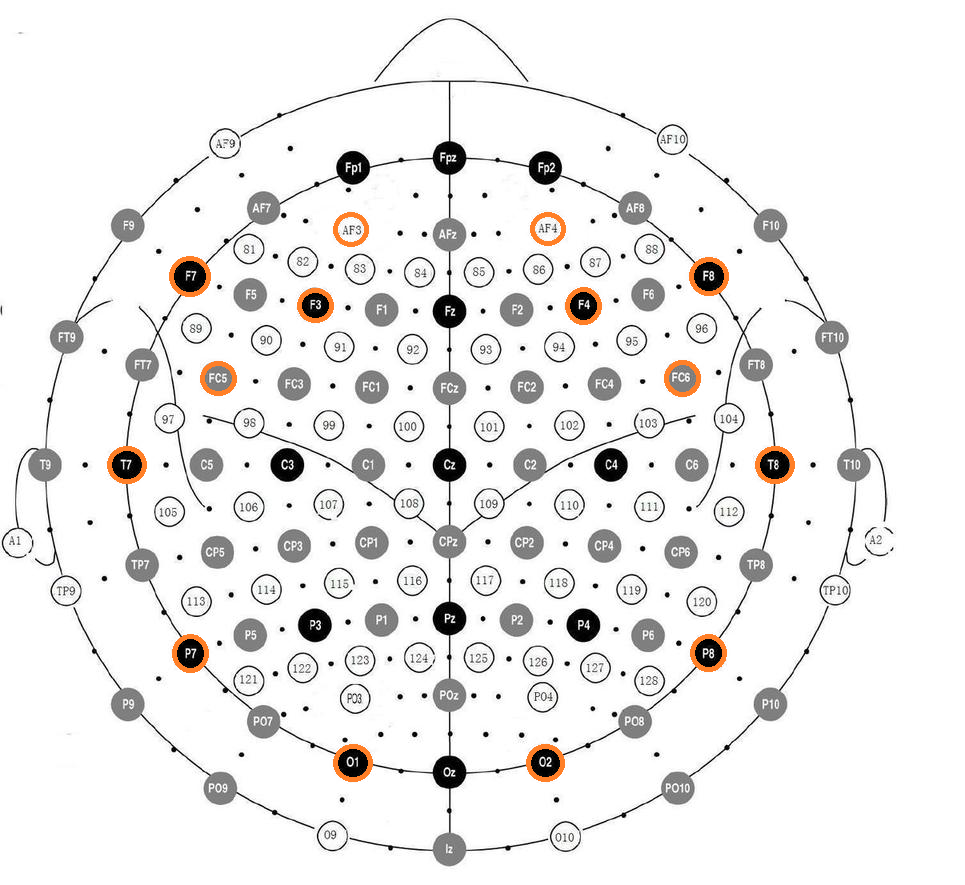
\includegraphics[width=0.6\textwidth]{electrode_locations.png}
	\caption{Electrode locations used by Emotiv EPOC\protect\footnotemark}
	\label{fig:electrode_locations}
\end{figure}
\footnotetext{http://emotiv.wikia.com/wiki/Emotiv\_EPOC}

Therefore, Emotiv EPOC is chosen as \gls{EEG} device for controlling a robot in this thesis. Chapter~\ref{sec:SSVEP_BCI} contains details about the designed application for controlling a robot.


\chapter{VEP-based brain-computer interface}

The previous chapter discussed the biology of the brain and described the brain potential called \gls{SSVEP}. The aim of this chapter is to describe which kind of visual stimuli can be used to elicit \gls{SSVEP} and how to detect \gls{SSVEP} in a \gls{EEG} recording. This knowledge is needed to extract information from the \gls{EEG} recording and use this information to control a robot. In other words, this chapter will discuss how to implement a \gls{VEP}-based \gls{BCI}.

\section{Visual stimulus}
\label{sec:stimuli}

As discussed in section~\ref{sec:VEP}, it is possible to present multiple visual stimuli to a subject and detect, which stimulus is the subject looking at. It was also mentioned that computer monitor can be used to present visual stimuli. This section will discuss how stimuli with certain blinking frequency can be displayed on a computer screen. Research has shown that LCD screens produce more reliable \gls{SSVEP} response than \gls{LED}~\cite{lcd_lcd_led}. Another article published in the same year, however, concludes that \glspl{BCI} that used \glspl{LED} as visual stimuli have achieved better performance~\cite{ssvep_stim}. But since using \glspl{LED} requires dedicated hardware, in this thesis only the stimulus that can be presented by a computer monitor is discussed.

A computer monitor has certain size, resolution and refresh rate. Monitor resolution and size limit the size of the visual stimuli that can be used and the distance between the stimuli. Monitor refresh rate, on the other hand, limits the blinking frequency of the stimulus that can be used. Research has shown that LCD screens produce more reliable \gls{SSVEP} response when using the monitor refresh rate for synchronisation rather than a timer~\cite{lcd_lcd_led}. In this thesis, monitor refresh rate is used for synchronisation.

Monitor refresh rate is the number of consecutive images or frames shown on screen in a second, assuming that the frames are produces at least as fast as they can be displayed. A frame is one of the images that compose the changing picture on screen. Monitor with a refresh rate of 60 Hz can display 60 frames per second. 

Often blinking one-coloured squares on one-coloured background are used as visual stimuli in \gls{SSVEP}-based \glspl{BCI}~\cite{ssvep_stim}. The squares may have symbols on them, for example letters or numbers. The stimuli of \gls{VEP}-based \gls{BCI} are also called \glspl{target}. The blinking of a target is called \gls{flickering}.

In every frame each \gls{target} can be in one of two states---displayed or not displayed. The state of a \gls{target} can be changed only when the frame changes. The state switches should be distributed as evenly as possible for the target frequency to be constant. Distributing the state switches is easier with some frequencies than others. For example, if refresh rate is 60 Hz, then
\begin{itemize}
	\item 10 Hz \gls{target} \gls{flickering} can be achieved by presenting the \gls{target} $\frac{60}{10}=6$ times slower than the refresh rate. This means, that the \gls{target} has to be presented once in every 6 frames. Since 6 is even number, 10 Hz \gls{flickering} can be achieved by changing the state of the \gls{target} after every 3 frames. If representing this \gls{flickering} as a waveform as in figure~\ref{fig:flickering}, it can be seen that the waveform is a \gls{square wave}.
	\item 12 Hz \gls{target} \gls{flickering} can be achieved by presenting the \gls{target} $\frac{60}{12}=5$ times slower than the refresh rate, the \gls{target} has to be presented once in every 5 frames and since 5 is odd number, the amount of time the target is in on state and in off state cannot be equal. Therefore, the \gls{target} should be 3 frames in displayed state and 2 frames in not displayed state or the other way round. If representing this \gls{flickering} as a waveform as in figure~\ref{fig:flickering}, it can be seen that the waveform is a \gls{rectangular wave}.
	\item 11 Hz \gls{target} \gls{flickering} can be achieved by presenting the \gls{target} $\frac{60}{11}\approx 5.45$ times slower than the refresh rate. This means, that the \gls{target} has to be presented once in every 5.45 frames. Since 5.45 is not a natural number, the \gls{target} \gls{flickering} will be irregular. 11 Hz target \gls{flickering} from the paper by Wang \textit{et al.}~\cite{11hz} is used as an example in figure~\ref{fig:flickering}. Although 11 Hz frequency produces irregular \gls{flickering}, it is still possible to detect \gls{SSVEP} elicited by it in the Emotiv EPOC recording~\cite{emotiv_11hz}. In this thesis, the waveform produced by 11 Hz \gls{flickering} is called an \gls{irregular square wave}.
\end{itemize}

\begin{figure}[h]
	\begin{subfigure}{\textwidth}
		\begin{tikztimingtable}[xscale=0.75, yscale=1.5, thick]
			10 Hz & [C] 10{3H 3L}\\
			11 Hz & [C] 11{2.73H 2.73L}\\
			12 Hz & [C] 12{2.5H 2.5L}\\
			\extracode
			\tablegrid[black!25,step=1]
		\end{tikztimingtable}
		\caption{Ideal target flickering}
	\end{subfigure}
	\begin{subfigure}{\textwidth}
		\begin{tikztimingtable}[xscale=0.75, yscale=1.5, thick]
			10 Hz & [C] 10{3H 3L}\\
			11 Hz & [C] 3H 3L 3H 2L 3H 3L 3H 2L 3H 3L 2H 3L 3H 3L 2H 3L 3H 3L 2H 3L 3H 2L\\
			12 Hz & [C] 12{3H 2L}\\
			\extracode
			\tablegrid[black!25,step=1]
		\end{tikztimingtable}
		\caption{Target flickering adjusted to refresh rate}
	\end{subfigure}
	\caption{Adjusting target flickering to refresh rate}
	\label{fig:flickering}
\end{figure}
A \gls{duty cycle} is used to characterise a \gls{rectangular wave}. \Gls{duty cycle} is the percentage of the amount of time the \gls{target} is in displayed state in one period. If the target is in displayed state for 2 frames and in not displayed state for 3 frames in one period, then the \gls{duty cycle} of the \gls{rectangular wave} is $\frac{2}{2+3}\cdot 100\%=40\%$. \Gls{square wave} has a duty cycle of 50\%. Research has shown that the \gls{SSVEP} elicited by \gls{square wave} \gls{flickering} can be more accurately detected than those elicited by \glspl{rectangular wave} \gls{flickering}.

The previous discussion was about blinking shapes or single graphic stimuli. There is another type of \gls{SSVEP} stimuli called pattern reversal stimuli that can also be presented by computer screen. Pattern reversal stimuli is rendered by changing between two different patterns, for example alternating the colours of a chequerboard~\cite{ssvep_stim}. The main difference between single graphic stimuli and pattern reversal stimuli is that single graphic stimuli elicits \gls{SSVEP} response after every two alterations, while pattern reversal stimuli elicits \gls{SSVEP} response after every alteration~\cite{ssvep_stim}.

The fastest possible target frequency can be achieved by changing between on and off states of the target every time a new frame is displayed. If the state is changed at lower rate, the \gls{target} frequency will also be lower. Perhaps it is most reasonable to calculate the \gls{target} frequency with:
\begin{equation}
	f_{single\mbox{ }graphic} = \frac{n}{2T} \qquad f_{pattern\mbox{ }reversal} = \frac{n}{T}
\end{equation}
where $T$ is the period of the \gls{flickering}, $n$ is the number of times the target state is switched in a time period of $T$ and $f$ is the target frequency.

\gls{SSVEP} reflects certain properties of the visual stimulus~\cite{ssvep_response}. Most important of these properties is that \gls{SSVEP} has a component with the same frequency as the visual stimulus. But that is not the only component frequency in \gls{SSVEP}. \gls{SSVEP} has other components too that are discussed in section~\ref{sec:fourier}. It is sufficient to detect only the component with visual stimuli presentation frequency in the \gls{EEG} recording, but to improve the performance other components should be detected too~\cite{harmonic_imrpovement}.

\section{Decomposing signals}

\subsection{Fourier analysis}
\label{sec:fourier}

As discussed in the previous section, the flickering of a target can produce different waveforms. This section will discuss how these waveforms and other signals can be represented by sums of simpler trigonometric functions. The study of this decomposition process is called Fourier analysis, named after Joseph Fourier, whose insight to model all functions by trigonometric series was a breakthrough in the field in 1807.

The following paragraph is based on the book by Hartmann~\cite{pure_tone}. The simpler trigonometric functions that a signal is decomposed into are pure tones---the waveforms that contain only one frequency. All other waveforms have at least two frequencies. Pure tone waveforms are sine and cosine waves. Important property of a pure tone is that linear operations do not change the shape of the pure tone waveform.

The pure tones are used to represent all possible frequencies that a signal may contain. The decomposition process of a signal is called Fourier transform and it is used to decompose a function of time into pure tones or frequency components that make it up. The function of time can be for example the \gls{EEG} recording represented as voltage versus time or the target flickering represented as state versus time. Fourier transform converts signal from time domain or the function of time to frequency domain or the function of frequency. The representation of a time-domain signal in a frequency domain is called frequency spectrum. Frequency spectrum contains information about amplitude and phase of different frequencies. Therefore, frequency spectrum can be presented as a function of frequency versus amplitude and phase.

To represent both amplitude and phase, complex numbers are used. Complex numbers can be represented as a pair of real numbers and therefore complex numbers can be used to represent two values. The amplitude and phase do not correspond to the real and imaginary part of the complex number but rather are related to the absolute value or the modulus and phase of the complex number. In this thesis the phase information from the frequency spectrum is not used. There are, however, \glspl{BCI} that also use phase information~\cite{MPCC}. Since only the information about amplitude is required in this thesis, it is possible to convert the frequency spectrum into power spectral density, which is represented as a function of amplitude squared or power versus frequency.

To conclude previous discussion, the amount of frequency $f$ present in a signal can be calculated by first calculating the frequency spectrum with Fourier transform and then taking modulus squared of the frequency spectrum's value at frequency $f$.

In digital devices, however, theoretical power spectral density cannot be calculated. The measurement period would have to be infinitely long to a acquire the true power spectral density~\cite{psd}. Therefore, power spectral estimation is used. The modulus squared of frequency spectrum in a real-world application is called periodogram and it is the estimation of the power spectral density. There are other spectral estimation methods available.

Since digital devices work with discrete signals as discussed in section~\ref{sec:EEG_comparison}, in a real-world application discrete version of the Fourier transform is used. The algorithm used to compute the discrete Fourier transform is called \gls{FFT}. The frequency spectrum calculated by \gls{FFT} is discrete---if the discrete real-valued input signal, as is the case with \gls{EEG} recording, has $N$ values then the output has $\frac{N}{2}$ values. This derives from the definition and symmetric property of the discrete Fourier transform. %The higher the sampling rate and \gls{ADC} resolution of a recording device, the more accurate the recording and therefore the more accurate the frequency spectrum and the periodogram of the signal.

The signal that is recorded, however, may contain frequencies that are too high to be detected from the discrete signal. Theoretically, the sampling rate of the device has to be more than two times higher than the highest frequency in the signal to reconstruct the continuous signal from the discrete signal or to decompose the signal into frequency components. When looking it from different angle, the highest frequency that can be detected with a sampling rate of $f$ is $\frac{2}{f}$ and it is called Nyguist frequency. But since real-world application are imperfect, even higher sampling rate are needed.

To conclude previous discussion, the frequency spectrum calculated by \gls{FFT} from real-valued time-domain signal with $N$ values is defined at frequencies $\frac{1}{N}, \frac{2}{N}, \dots\frac{f}{2N}$. These frequencies are also called frequency bins. The length of a frequency spectrum depends on the length of the signal from which it is calculated. The longer the signal, the more frequency bins will be acquired.

Thus a time-domain signal can be decomposed into pure tones or sine and cosine waves using \gls{FFT}. \gls{FFT} calculates the frequency spectrum of a time-domain signal. Frequency spectrum can be converted to the estimation of power spectral density which contains only the information about the amplitude of the pure tones. This knowledge can be used to detect \glspl{SSVEP} in \gls{EEG} recording.

%As already discussed in section~\ref{sec:EEG_comparison}, Emotiv EPOC has high internal sampling rate to filter out high frequencies

%Thus higher sampling rate and \gls{ADC} resolution lead to more accurate \gls{SSVEP} detection.

\subsection{Decomposition of target flickering}

It can be shown that a square wave is composed of the \gls{fundamental} frequency and its odd \glspl{harmonic}. \Gls{fundamental} frequency is the component with lowest frequency among the components that make up the wave. In case of \gls{square wave} \gls{flickering} and \gls{rectangular wave} \gls{flickering}, the \gls{fundamental} frequency is the frequency of the stimuli presentation. \Glspl{harmonic} are the components of a signal that have frequency of a multiple of the fundamental frequency of the same signal. Therefore, \gls{square wave} can be represented as a sum of sine waves
\begin{equation}
	\label{eq:square}
	square(x) = \sum_{i=1}^{\infty}a_i sin(2\pi 2if)
\end{equation}
where $square(x)$ is the flickering represented as state versus time, $f$ is the flickering frequency and $a_i$ is the amplitude of i'th component. \Gls{fundamental} frequency of a square wave or rectangular wave has the highest amplitude or in other words, $\max_i a_i=a_1$. \Gls{rectangular wave}'s frequency depends on the \gls{duty cycle} of the wave.

Unfortunately, the \gls{SSVEP} response to \gls{target} \gls{flickering} does not contain only the frequencies present in the waveform of the \gls{target} \gls{flickering}, but the frequencies that are present in the components of \gls{target} \gls{flickering} are more successfully elicited in \gls{SSVEP}~\cite{square_sine}. It has even been reported that \gls{SSVEP} contains small subharmonics of the fundamental frequency.
%Rectangular wave is composed of frequencies not including every third harmonic
%\begin{equation}
%	rectangular(x)=\sum_{i=1}^{\infty} a_i sin(2\pi if)+b_i sin(2\pi 2if)
%\end{equation}

\section{Related work}

There are many types of \glspl{BCI} available. A review by Bashashati \textit{et al.}~\cite{bci_comparison} contains a detailed overview of \gls{EEG}-based \glspl{BCI}. Their paper includes overview of the following neuromechanisms used in \gls{EEG}-based \glspl{BCI}: \gls{VEP} and \gls{SSVEP}, P300, slow cortical potential, response to mental task, sensorimotor activity, and multiple neuromechanisms or hybrid \gls{BCI}. Hybrid \gls{BCI} uses two different neuromechanisms in a \gls{BCI} and therefore two different methods are required to analyse \gls{EEG} recording~\cite{hybrid_bci, hybrid_bci2}. %In this thesis, main focus is on \gls{SSVEP}-based \glspl{BCI}. 

\gls{SSVEP}-based \glspl{BCI} can be divided in categories according to the method used to detect \glspl{SSVEP} in \gls{EEG} recording. These methods are also called \gls{feature extraction} methods. Current \gls{SSVEP}-based \gls{BCI} \gls{feature extraction} methods include:
\begin{itemize}
	\item \Gls{PSDA} method introduced by Cheng \textit{et al.}~\cite{psda}.
	\item \Gls{SC} method introduced by Wu and Yao~\cite{sc}.
	\item Dual-frequency \gls{SSVEP} methods~\cite{dual1, dual2}.
	\item \Gls{MPCC} method introduced by Tong \textit{et al.}~\cite{MPCC}.
	\item \Gls{MEC} method introduced by Friman \textit{et al.}~\cite{mec}. This method has shown better performance than \gls{SC} and \gls{PSDA} method~\cite{mec_comparison}.
	\item \Gls{CCA} method introduced by Lin \textit{et al.}~\cite{cca_lin}. This method has shown better performance than \gls{PSDA} method~\cite{cca_psda, bin2009cca, cca_lin}.
	\item \Gls{LASSO} method introduced by Zhang \textit{et al.}~\cite{LASSO}. This method has shown better performance than \gls{CCA} method~\cite{LASSO}.
	\item \Gls{LRT} method introduced by Zhang \textit{et al.}~\cite{LRT}. This method has shown better performance than \gls{CCA} method and similar performance to \gls{LASSO} method~\cite{LRT}.
\end{itemize}
There is also an improvement of \gls{CCA} method available called multiway \gls{CCA}, which has shown slightly better performance than standard \gls{CCA} method~\cite{mcca}.

In this thesis, Emotiv EPOC is used to record brain activity. The following papers also describe \glspl{BCI} that used Emotiv EPOC to record brain activity:
\begin{itemize}
	\item Liu \textit{et al.}~\cite{emotiv_11hz} used \gls{CCA} method;
	\item Lin \textit{et al.}~\cite{emotiv_walking} used \gls{CCA} method;
	\item Choi and Jo~\cite{emotiv_hybrid} designed hybrid \gls{BCI};
	\item Zier~\cite{emotiv_psda} used \gls{PSDA} method;
	\item Hvaring and Ulltveit-Moe~\cite{emotiv_comparison} compared different \gls{feature extraction} methods using Emotiv EPOC;
	\item Duvinage \textit{et al.}~\cite{emotiv_p300_comp} used P300 method and compared the performance of Emotiv EPOC and a medical-grade device.
\end{itemize}
%This thesis focuses on two of these methods: \gls{PSDA} and \gls{CCA} methods.


\section{SSVEP-based brain-computer interface}
\label{sec:SSVEP_detection}
The aim of this chapter is to describe two methods used to detect \glspl{SSVEP} in \gls{EEG} recording. 
This section describes the \gls{PSDA} and \gls{CCA} method. These are the methods used in chapter~\ref{sec:SSVEP_BCI} to design application for controlling a robot. 

\subsection{Power spectral density analysis}

\Gls{PSDA} is widely used in \gls{SSVEP}-based \glspl{BCI}~\cite{bin2009cca}. This method is uses \gls{FFT} to estimate power spectral density. The power spectral estimation calculated by taking the absolute value squared of the \gls{FFT} is called periodogram. 

\subsection{Canonical correlation analysis}

\Gls{CCA} was first introduced by Harold Hotelling in 1936~\cite{cca_hotelling}. In 2001 \gls{CCA} was used to introduce a novel method for detecting neural activity in \gls{fMRI} data~\cite{cca_fmri}. Likewise, \gls{CCA} was introduced to \gls{EEG} recording analysis for the first time in 2007~\cite{cca_lin}. 

\Gls{CCA} is statistical method that can be used when analysing two sets of data. In \gls{SSVEP}-based \glspl{BCI} one set of data is the multichannel \gls{EEG} recording. For example, if recording data with electrodes located in O1 and O2, the recorded data can be represented with canonical variable~$X=x_{O1}+x_{O2}$. The second set of data is the \gls{fundamental} frequency and \glspl{harmonic} of the \gls{flickering} frequency. Both sine and cosine waves are used in the second data set % since the phase of the \gls{SSVEP} is not known.
\begin{equation}
	\label{eq:cca_ref}
	Y=\left(\begin{matrix}
		sin(2\pi)\\
		cos(2\pi)\\
		sin(2\pi)\\
		cos(2\pi)\\
		sin(2\pi)\\
		cos(2\pi)\\
	\end{matrix}\right)
\end{equation}
In the method proposed by ... \textit{et al.} three harmonics are used as in equation~\ref{eq:cca_ref}.


\chapter{Application for controlling a robot via SSVEP}
\label{sec:SSVEP_BCI}

The aim of this chapter is to describe the \gls{SSVEP}-based \gls{BCI} designed as a practical part of this thesis. The \gls{BCI} is written in Python 2.7 and the code is accessible from Github repository\footnote{https://github.com/kahvel/VEP-BCI}. The \gls{BCI} requires only Emotiv EPOC headset and a computer with Windows operating system, no specific hardware like digital signal processors or \glspl{LED} are used.

\section{Related work}

There are many types of \glspl{BCI} available. A review by Bashashati \textit{et al.}~\cite{bci_comparison} contains a detailed overview of \gls{EEG}-based \glspl{BCI}. Their paper includes overview of the following neuromechanisms used in \gls{EEG}-based \glspl{BCI}: \gls{VEP} and \gls{SSVEP}, P300, slow cortical potential, response to mental task, sensorimotor activity, and multiple neuromechanisms or hybrid \gls{BCI}. Hybrid \gls{BCI} uses at least two different neuromechanisms in a \gls{BCI} and therefore at least two different methods are required to analyse the \gls{EEG} recording~\cite{hybrid_bci, hybrid_bci2}.

\gls{SSVEP}-based \glspl{BCI} can be divided in categories according to the method used to detect \glspl{SSVEP} in \gls{EEG} recording. Current \gls{SSVEP}-based \gls{BCI} \gls{feature extraction} methods include:
\begin{itemize}
	\item \Gls{PSDA} method introduced by Cheng \textit{et al.}~\cite{psda}.
	\item \Gls{SC} method introduced by Wu and Yao~\cite{sc}.
	\item Dual-frequency \gls{SSVEP} methods~\cite{dual1, dual2}.
	\item \Gls{MPCC} method introduced by Tong \textit{et al.}~\cite{MPCC}.
	\item \Gls{MEC} method introduced by Friman \textit{et al.}~\cite{mec}. This method has shown better performance than \gls{SC} and \gls{PSDA} method~\cite{mec_comparison}.
	\item \Gls{CCA} method introduced by Lin \textit{et al.}~\cite{cca_lin}. This method has shown better performance than \gls{PSDA} method~\cite{cca_psda, bin2009cca, cca_lin}.
	\item Multiway \gls{CCA} method introduced by Zhang \textit{et al.}~\cite{mcca}. This method has shown better performance than standard \gls{CCA}~\cite{mcca}.
	\item \Gls{LASSO} method introduced by Zhang \textit{et al.}~\cite{LASSO}. This method has shown better performance than \gls{CCA} method~\cite{LASSO}.
	\item \Gls{LRT} method introduced by Zhang \textit{et al.}~\cite{LRT}. This method has shown better performance than \gls{CCA} method and similar performance to \gls{LASSO} method~\cite{LRT}.
\end{itemize}
For more comprehensive review of the \gls{feature extraction} methods see article by Liu \textit{et al.}~\cite{feature_extraction}.

In this thesis, Emotiv EPOC is used to record brain activity. Table~\ref{tab:emotiv_BCIs} gives overview of the existing \glspl{BCI} that also use Emotiv EPOC for recording brain activity. It can be seen that existing applications have \gls{target} detection time above or exactly three seconds which is not fast enough to control a robot in real time. However, as Zier mentioned in his paper~\cite{emotiv_psda} and as also noticed in the process of developing this application, if the \gls{window} length is long enough for the \gls{feature extraction} method to accurately detect correct \gls{target}, the \gls{target} detection time is about half the \gls{window} length. That is so, because after half the \gls{window} length, half of the previous data is replaced with new data and if there is more new data than previous, then the \gls{BCI} recognises the new user's choice.

\newcommand{\liu}{Liu \textit{et al.}~\cite{emotiv_11hz}}
\newcommand{\lin}{Lin \textit{et al.}~\cite{emotiv_walking}}
\newcommand{\choi}{Choi and Jo~\cite{emotiv_hybrid}}
\newcommand{\hvar}{Hvaring and}
\newcommand{\moe}{Ulltveit-Moe~\cite{emotiv_comparison}}
\newcommand{\duvi}{Duvinage \textit{et al.}~\cite{emotiv_p300_comp}}

\begin{table}[h]
	\centering
	\begin{tabular}{|c|c|c|c|c|}\hline
		& Method& Accuracy (\%)		& Target detection 	& ITR (bits/min)	\\
		&		&					& time (sec)		&					\\\hline
\liu	& CCA	& $95.83\pm 3.59$	& $5.25\pm 2.14$	& $20.97\pm 0.37$	\\\hline
\lin	& CCA	& $76.60\pm 21.74$	& $4.34\pm 0.08$	& $14.38\pm 9.04$	\\\hline
		& CCA	& $84.4\pm 5.0$		& N/A				& $11.6\pm 3.9$		\\\cline{2-5}
\choi	& ERD	& $84.6\pm 5.3$		& N/A				& $11.8\pm 3.7$		\\\cline{2-5}
		& P300	& $89.5$			& $5.35$			& $18.1\pm 2.1$		\\\hline
\hvar	& CCA	& $85.12\pm 4.58$	& $3.00$			& $32.92\pm 4.72$	\\\cline{2-5}
\moe	& PSDA	& $89.29\pm 6.41$	& $5.14\pm 0.98$	& $23.78\pm 7.15$	\\\hline
	\end{tabular}
	\caption{Comparison of the existing BCIs that use Emotiv EPOC.}
	\label{tab:emotiv_BCIs}
\end{table}

This thesis aims at developing \gls{BCI} with faster \gls{target} detection time than the previous applications to provide suitable speed for controlling a robot.
%This thesis focuses on two of these methods: \gls{PSDA} and \gls{CCA} methods.

\section{Overview of the application}
\label{sec:application}

As already mentioned, the application is written in Python 2.7. In addition to the Python 2.7 standard library, the following libraries were used:
\begin{itemize}
	\item Emokit\footnote{https://github.com/openyou/emokit/tree/master/python/emokit} to access raw data from Emotiv EPOC headset;
	\item PsychoPy~\cite{psychopy} for designing visual stimuli and precise timing of the stimuli presentations;
	\item scikit-learn~\cite{scikit-learn} for calculating \gls{CCA} algorithm;
	\item SciPy and NumPy~\cite{scipy} for calculating other advanced mathematical algorithms, for example \gls{FFT};
	\item PyQtGraph\footnote{http://www.pyqtgraph.org} for real-time plotting of the data.
\end{itemize} For the ease of use, the application has graphical user interface. See figure~\ref{fig:options_frame} for an example the application's user interface.

The application runs on multiple subprocesses and therefore is able to use multiple \glspl{CPU} or multiple \gls{CPU} cores at the same time. This is achieved by using Python multiprocessing module. Multiprocessing is also important to avoid freezing of the whole application while one window is moved or resized, since this is the default behaviour of the window manager of Windows operating system. The components of the application that run on different processes can be seen in figure~\ref{fig:class_diagram}.

\begin{figure}[h!]
	\centering
	\tikzstyle{decision} = [diamond, draw, fill=blue!20,
    text width=4.5em, text badly centered, node distance=2.5cm, inner sep=0pt]
\tikzstyle{block} = [rectangle, draw, fill=blue!20,
    text width=5em, text centered, rounded corners, minimum height=4em]
\tikzstyle{line} = [draw, very thick, color=black!50]
\tikzstyle{cloud} = [draw, ellipse,fill=red!20,
    minimum height=2em]

\newcommand*{\ArrowLength}{2.0em}
\newcommand*{\MyRightArrow}[1][]{
    \tikz [-stealth, red, yshift=0.5ex, baseline] 
        \draw [-stealth, #1] (0,0) -- (\ArrowLength,0) ;
}

\begin{tikzpicture}[scale=2, node distance = 4cm, auto]
	% Nodes
	\node [block] (PostOffice) {\texttt{PostOffice}};
	\node [block, left of=PostOffice] (MainWindow) {\texttt{Main Window}};
	\node [block, right of=PostOffice] (TargetsWindow) {\texttt{Targets Window}};
	\node [block, below of=TargetsWindow, node distance=2cm] (Robot) {\texttt{Robot}};
	\node [block, below of=MainWindow, node distance=2cm] (MyEmotiv) {\texttt{Emotiv}};
	\node [block, above of=TargetsWindow, node distance=2cm] (Plot) {\texttt{Plot}};
	\node [block, above of=MainWindow, node distance=2cm] (Extraction) {\texttt{Extraction}};
	
	% Arrows
	\path [line] (PostOffice) -- node [pos=0.1, above, color=black] {1} node[pos=0.9, above, color=black] {1} (MyEmotiv);
	\path [line] (PostOffice) -- node [pos=0.1, above, color=black] {1} node[pos=0.9, above, color=black] {1} (TargetsWindow);
	\path [line] (PostOffice) -- node [pos=0.1, above, color=black] {1} node[pos=0.9, above, color=black] {1} (MainWindow);
	\path [line] (PostOffice) -- node [pos=0.1, above, color=black] {1} node[pos=0.9, above, color=black] {1} (Robot);
	\path [line] (PostOffice) -- node [pos=0.1, above, color=black] {1} node[pos=0.9, above, color=black] {n} (Plot);
	\path [line] (PostOffice) -- node [pos=0.1, above, color=black] {1} node[pos=0.85, above, color=black] {m} (Extraction);

\end{tikzpicture}

	\caption{Components of the application.}
	\label{fig:class_diagram}
\end{figure}

The communication between different components is implemented using multiprocessing connections. Each line in figure~\ref{fig:class_diagram} represents one connection. It can be seen that all the connections go to the PostOffice class. This class is used to receive and send messages between different components of the application.

\section{Using the application with other EEG devices}
\label{sec:different_devices}

Although the application was written for Emotiv EPOC, it can be used with other \gls{EEG} devices too if it is possible to access the data of these devices with Python script. As discussed in section~\ref{sec:application}, the communication between the data accessing code and the rest of the application is realised using Python multiprocessing module. The data accessing code runs on separate process and communicates with the rest of the application by sending messages through multiprocessing connection. It sends raw data through the connection and receives messages like "Setup", "Start", "Stop" and "Exit". Each of the received messages should lead to calling a specific function. If the received message is
\begin{itemize}
	\item "Setup", then the object should get internally ready to start sending data;
	\item "Start", then the object should start sending the data;
	\item "Stop", then the object should stop sending the data;
	\item "Exit", then all the needed clean up procedures should be executed, because the application is closing.
\end{itemize}

The easiest way to start using different headset with the application is changing the code in MyEmotiv.py. The constructor of MyEmotiv class has to take one argument. This argument is the object that handles the communication between different processes. The last line in the constructor of MyEmotiv should call the argument's waitMessages method, which waits until it receives one of the previously discussed messages. The waitMessages method takes arguments which are the functions that are called when corresponding message is received. By replacing these methods in MyEmotiv object, it is possible to use the application with other \gls{EEG} devices too. Since the application can be relatively easily modified to use other \gls{EEG} devices too, it could be a good tool to test how suitable are different devices for a \gls{SSVEP}-based \gls{BCI}.

\section{Signal pipeline of the application}
\label{sec:signal_pipeline}

The application does not have one specific signal pipeline, but the components of the pipeline can be changed using the graphical user interface. This allows different configurations to be easily tested to find the best settings for controlling a robot and the best settings for different users. See figure~\ref{fig:signal_pipeline} for the flowchart of the application's signal pipeline.

\begin{figure}[h!]
	\tikzstyle{decision} = [diamond, draw, fill=blue!20,
    text width=4.5em, text badly centered, node distance=2.5cm, inner sep=0pt]
\tikzstyle{block} = [rectangle, draw, fill=blue!20,
    text width=5em, text centered, rounded corners, minimum height=4em]
\tikzstyle{line} = [draw, very thick, color=black!50, -latex']
\tikzstyle{cloud} = [draw, ellipse,fill=red!20, node distance=3cm,
    minimum height=2em]

\begin{tikzpicture}[scale=2, node distance = 4cm, auto]
	% Nodes
	\node [cloud] (start) {start};
	\node [decision, below of=start] (wait) {wait for step packets};
	\node [block, right of=wait] (filter) {filter new signal segment};
	\node [cloud, right of=start] (stop) {stop};
	\node [block, right of=filter] (add) {add segment to signal};
	\node [decision, right of=add, node distance=4 cm] (length) {len(signal) \textgreater window length?};
	\node [block, below of=length] (delete) {delete first step packets};
	\node [block, left of=delete] (detrend) {make copy of signal and detrend it};
	\node [block, left of=detrend] (window) {window signal};
	\node [block, left of=window] (detect) {send signal to feature extraction};
	
	% Arrows
	\path [line] (start) -- (wait);
	\path [line] (wait) -- node [align=center, color=black, sloped, pos=1] {received\\"Stop"} (stop);
	\path [line] (wait) -- node [align=center, color=black, sloped] {received\\data} (filter);
	\path [line] (filter) -- (add);
	\path [line] (add) -- (length);
	\path [line] (length) -- node [near start, color=black] {yes} (delete);
	\path [line] (length) -- node [near start, color=black] {no} (detrend);
	\path [line] (detrend) -- (window);
	\path [line] (delete) -- (detrend);
	\path [line] (window) -- (detect);
	\path [line] (detect) -- (wait);
\end{tikzpicture}

	\caption{Flowchart of the application's signal pipeline.}
	\label{fig:signal_pipeline}
\end{figure}

As seen in figure~\ref{fig:signal_pipeline}, all the signal processing techniques discussed in section~\ref{sec:signal_processing} can be used as components of the signal pipeline and in addition to these techniques, filtering can also be used. One thing to keep in mind is that the \gls{window} length shows how long signal is held in memory and after every step, the whole signal goes through the signal pipeline, not only the segment obtained during the last step. See figure~\ref{fig:options_frame} for illustration of the application's user interface for choosing signal pipeline components and options.

\begin{figure}[h]
	\centering
	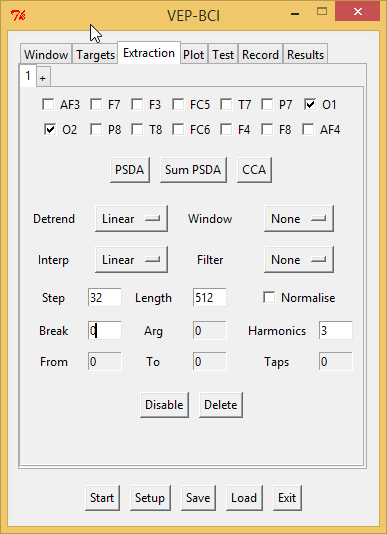
\includegraphics[width=0.6\textwidth]{options_frame.png}
	\caption{The user interface for choosing signal pipeline options.}
	\label{fig:options_frame}
\end{figure}

The explanation of the signal pipeline options is the following:
\begin{enumerate}
	\item \Gls{detrend} is either linear, constant or none. None means that \glsdisp{detrend}{detrending} is not used. Linear means that linear trend is removed from the raw signal; constant means that constant trend is removed from the raw signal. \glsdisp{detrend}{Detrending} was more thoroughly discussed in section~\ref{sec:detrend}.
	\item \Gls{window} is either hann, hamming, blackman, keiser, bartlett or none. None means that \gls{window} function is not used. Other options are standard signal processing \gls{window} functions. \glsdisp{window}{Windowing} was more thoroughly discussed in section~\ref{sec:window}.
	\item \glsdisp{interpolation}{Interp} is either linear, nearest, zero, slinear, quadratic or cubic. See SciPy documentation\footnote{https://docs.scipy.org/doc/scipy/reference/generated/scipy.interpolate.interp1d.html} for more information. \Gls{interpolation} was more thoroughly discussed in section~\ref{sec:interpolate}.
	\item Filter is either high-pass, low-pass, band-pass or none. None means that filtering is not used. High-pass filter means that frequencies lower than the given value are removed from the signal. Similarly, low-pass filter removes frequencies higher than the given value. Band-pass filter takes two values and removes frequencies that are not in the given range. See SciPy documentation\footnote{http://docs.scipy.org/doc/scipy/reference/generated/scipy.signal.firwin.html} for more information. 
	\item Step shows how many packets have to be received before trying to identify user's choice. For example, if \gls{sampling rate} is \SI{128}{Hz} and step is 64 then the \gls{feature extraction} algorithms are executed after every $\frac{64}{\SI{128}{Hz}}=0.5$ seconds.
	\item Length is the length of the window. Length shows the number of packets on which the \gls{feature extraction} algorithms are executed. For example, if \gls{sampling rate} is \SI{128}{Hz} and length is 512 then the \gls{feature extraction} algorithms are performed on the last $\frac{512}{\SI{128}{Hz}}=4$ seconds of data.
	\item Break is the number of breakpoints used when \glsdisp{detrend}{detrending} the signal. The breakpoints will be equally spaced. If the number of breakpoints is 1, then the breakpoint will be in the middle of the signal and the trend will be removed separately from the first half of the signal and the second half of the signal.
	\item Arg is the beta argument for kaiser window. See NumPy documentation for details\footnote{http://docs.scipy.org/doc/numpy/reference/generated/numpy.kaiser.html}.
	\item Harmonics is the number of integer multiples used in \gls{feature extraction} methods. How integer multiples of the \gls{target} frequency can be used in \gls{PSDA} and \gls{CCA} methods was discussed in sections~\ref{sec:PSDA} and \ref{sec:CCA} respectively. The motivation for using integer multiples was discussed in section~\ref{sec:decomposition}.
	\item Normalise shows whether to normalise the estimated \gls{power spectral density} as in equation~\ref{eq:norm_SNR} or not.
	\item From and to are the frequencies used to specify which frequencies are removed and which not. From shows the lowest frequency that is passed, lower frequencies than the value will be removed; to shows the highest frequency that is passed, higher frequencies than the value will be removed.
	\item Taps shows the number of taps or the length of the filter. See SciPy documentation\addtocounter{footnote}{-2}\footnotemark\addtocounter{footnote}{1} for details.
\end{enumerate}

The application has graphical user interface and the code is written so that it is relatively easy to add new or change the existing functionality, as briefly discussed in section~\ref{sec:different_devices}. This application can be used to compare how different signal pipelines affect the detection of \glspl{SSVEP}.

\section{Target identification method}
\label{sec:identification}

This section describes the user's choice identification method used in this application. As is the case with the signal pipeline, this application actually does not have one specific \gls{feature extraction} method, but the \gls{feature extraction} method can be changed and a combinations of different \gls{feature extraction} methods can be used. To the best of the author's knowledge, combining different \gls{feature extraction} methods while using only \gls{SSVEP} neuromechanism has not been used before.

Currently the application has three different \gls{feature extraction} methods that can be combined: widely known \gls{PSDA} and \gls{CCA} method and a method that is similar to the \gls{PSDA} method but the estimated \gls{power spectral density} is calculated not for each signal obtained from different channels but for the sum of all the signals from different channels. If only one channel is used, then this method works exactly the same as standard \gls{PSDA} method. In the graphical user interface, this method is called sum \gls{PSDA} method. Using this method makes sense, because \gls{FFT} is linear, meaning that the result will be the same if first the signals are summed up and then the \gls{power spectral density} is estimated and if first the \gls{power spectral density} is estimated separately for each channel and then the \gls{power spectral density} estimates for each channel are summed up.

Unlike the sum \gls{PSDA} method, the standard \gls{PSDA} method calculates separate results for each channel. One way to identify user's choice with standard \gls{PSDA} method is to choose a command only if all the \gls{PSDA} methods give the same result. If all the methods do not give the same result, it is assumed that the signal was too noisy and the decision could not be made. In this case the application waits for new data.

All \gls{feature extraction} methods used in the application can be combined. In case of combining methods, the \gls{target} choosing algorithm is similar to the standard \gls{PSDA} method---all the methods have to give the same result. Currently the \gls{target} choosing method cannot be changed from the user interface. If different \gls{target} choosing method is needed, then the code has to be changed.

It is easy to modify this functionality by changing the code in handleFreqMessage method in PostOffice.py. This method receives the results of the \gls{feature extraction} methods through a connection similarly to the data accessing code discussed in section~\ref{sec:different_devices}. The results have already been organised into different data structures. There are results per each method, results per each signal pipeline, all the results counted and other data structures to make it easier to further develop the application.

It is also worth mentioning that different \gls{feature extraction} methods can have different signal pipelines. For example it would not make sense to \gls{window} a signal that is later analysed using \gls{CCA}, but \glsdisp{window}{windowing} could be beneficial if the estimated \gls{power spectral density} of the signal is later analysed using \gls{PSDA} method. Thus the application has the functionality to use multiple signal pipelines with different options, which gives even more flexibility.

Using \gls{PSDA} and \gls{CCA} method together makes the \gls{target} identification more accurate, because finally the \gls{target} is chosen only if different methods give the same result. If one of the methods makes a mistake and gives a wrong result, then the other method might still give the correct result. It is less probable for two methods to make the same mistake at the same time than for one method to make a mistake. Using these two methods together makes sense, because these methods analyse the \gls{EEG} signal from two different aspects---one uses time-domain representation, the other uses frequency-domain representation.

To further improve this method, the phase information from the \gls{frequency spectrum} that is currently being discarded could also be used. One possible usage would be to design \gls{CCA} method \glspl{reference signal} with correct phase. Currently both sine and cosine waves are used to achieve optimal minimum correlation as discussed in section~\ref{sec:CCA}. But even without this improvement, combining these methods already improves the performance of the \gls{BCI}.

\section{Controlling a robot with the application}

As discussed in section~\ref{sec:identification}, the application does not have one specific \gls{feature extraction} method but it combines different \gls{feature extraction} methods with different signal pipelines if necessary. Thus the way how the signal is processed and how the user's choice is identified is modifiable. This section describes how the \gls{BCI} can be used to control a robot.

Each \gls{target} in the \gls{BCI} can be used as one command for the robot. The robot can be controlled by looking at different \glspl{target} on the computer screen in certain sequence, depending on which command should be given to the robot. Then the \gls{BCI} tries to identify which \gls{target} is being looked at and translates the results into commands for the robot, for example forward, left, forward. The \glspl{target} could be designed for example as shown in figure~\ref{fig:arrow_stimuli}.

\begin{figure}[h]
	\centering
	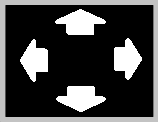
\includegraphics[width=0.4\textwidth]{arrows.png}
	\caption{Stimuli locations on the screen for controlling a robot.}
	\label{fig:arrow_stimuli}
\end{figure}

The robot\footnote{https://github.com/kuz/Garage48-PiTank} used for testing the application has five possible commands move forward, move backward, turn left, turn right and stop. The robot can execute one command at a time, meaning that it is not possible to move forward and turn left or right at the same time. If the robot is moving forward and receives different command, the moving forward will stop. See figure~\ref{fig:robot} for a picture of the robot used for testing the application.

\begin{figure}[h]
	\centering
	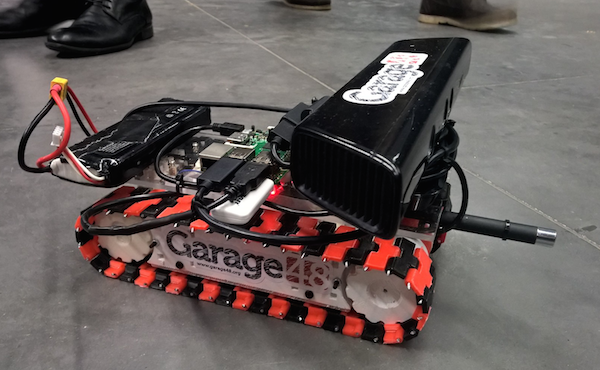
\includegraphics[width=0.6\textwidth]{robot.png}
	\caption{The robot used for testing the application\protect\footnotemark.}
	\label{fig:robot}
\end{figure}
\footnotetext{https://github.com/kuz/Garage48-PiTank/blob/master/Docs/images/pitank.png}
The robot has a camera on it and thus it is possible to see the camera's videos stream on the computer screen when controlling the robot with the application. The empty space in the middle of the screen as shown in figure~\ref{fig:arrow_stimuli} is intended---it is possible to show the video stream there.

The communication between the robot and the application is implemented similarly to the communication between other parts of the application, but instead of multiprocessing connections, sockets were used to exchange information.

[TODO: Add other details of the implementation if needed (not done yet, Ilya is searching for a camera for the robot)].

[TODO: Add the ITR/accuracy/speed and compare to existing BCIs]


\chapter{Results}

\addcontentsline{toc}{chapter}{Conclusion}

\chapter*{Conclusion}

The aim of this thesis has been to describe an \gls{SSVEP}-based \gls{BCI} implemented as a practical part of this thesis. In the first chapter the biological background was discussed to understand how brain activity can be measured and a low-cost \gls{EEG} device called Emotiv EPOC was chosen for recording the brain activity.

The second chapter provided an overview of the mathematical and technological background. Widely used \gls{feature extraction} methods called \gls{PSDA} and \gls{CCA} were discussed in this chapter along with signal processing techniques. All the discussed \gls{feature extraction} methods and signal processing techniques were used in the implemented application.

Finally, the third chapter described the implemented application itself. The strengths of the application compared to the existing applications are that this application is open-source, it allows different options for signal pipeline to be easily tested and it combines different \gls{SSVEP} \gls{feature extraction} methods. Although there are hybrid \glspl{BCI} that use different neuromechanisms and therefore these \glspl{BCI} use different \gls{feature extraction} methods, to the best of the author's knowledge there are no \glspl{BCI} that use different \gls{feature extraction} methods with one neuromechanism, in this case \gls{SSVEP}.

The application could be further developed to support different \gls{EEG} devices and more \gls{feature extraction} methods to find the best combination of different \gls{feature extraction} methods. Using multiple methods at the same time clearly improves the performance of a \gls{BCI}, but on the other hand it is computationally more expensive. But as the technology improves, this becomes less relevant.

[TODO: after measuring the performance of my application, add a paragraph about the that somewhere]



% References
% styles: https://www.sharelatex.com/learn/Bibtex_bibliography_styles

\bibliographystyle{abbrv}
\addcontentsline{toc}{chapter}{References}
\bibliography{thesis}
Internet URLs were valid on ...

% Appendices
% Can be replaced by \appendix

\begin{appendices}
\setcounter{table}{0}
\renewcommand{\thetable}{A\arabic{table}}
%\titleformat{\chapter}{\large\bfseries}{\appendixname~\thesection .}{0.5em}{}
%\titleformat{\chapter}{\normalfont\LARGE\bfseries}{\appendixname~\thechapter}{20pt}{}{}
\renewcommand{\thesection}{\Roman{section}}
\section{Glossary}
\printglossary
\newpage
\section{Acronyms}
\printglossary[type=\acronymtype]
\newpage
\begin{landscape}
\section{Fixed parameters for testing}
\label{sec:parameters}
	\begin{table}[h]
		\centering
		\begin{tabular}{|l|l|l|l|l|l|l|l|l|l|l|}\hline
Method& Extraction& Length& Step	& Sensors		& Detrend	& Detrend	 & Window& Kaiser& Interpolation& Filter\\
ID	& method	& (sec)	& (sec)	& 				& 			& breakpoints& 		 & beta	 & 				&  \\\hline
1	& Sum PSDA	& 2		& 0.125	& O1, O2		& Linear	& 5			 & Kaiser& 14	 & Quadratic	&- \\\hline
2	& CCA		& 2		& 0.125	& O1, O2, P7, P8& Linear	& 5			 & -	 & -	 & -			&- \\\hline
3	& PSDA		& 1		& 0.125	& O1, O2		& Linear	& 3			 & Kaiser& 14	 & Quadratic	&- \\\hline
4	& CCA		& 1		& 0.125	& O1, O2, P7, P8& Linear	& 3			 & -	 & -	 & -			&- \\\hline
		\end{tabular}
		\caption{Settings of the feature extraction method's signal pipelines.}
		\label{tab:pipelines}
	\end{table}
	\begin{table}[h]
		\centering
		\begin{tabular}{|l|l|l|l|l|l|l|l|l|l|}\hline
Target	& Frequency & Harmonics		& Position x& Position y& Color	& Type			& Shape	 & Width 	& Height\\
ID		& (Hz)		& in extraction	& (pixel)	& (pixel)	& 		& 		 		& 		 & (pixel)	&(pixel)\\\hline
1		& 5.45		& 1, 2, 3		& 0		 	& -200		& White	& Single graphic& Square & 150	 	& 150\\\hline
2		& 6.0		& 1, 2, 3		& -300	 	& 0			& White	& Single graphic& Square & 150	 	& 150\\\hline
3		& 6.67		& 1, 2, 3		& 0		 	& 200		& White	& Single graphic& Square & 150	 	& 150\\\hline
4		& 7.5		& 1, 2, 3		& 300	 	& 0			& White	& Single graphic& Square & 150	 	& 150\\\hline
		\end{tabular}
		\caption{Settings of the targets.}
		\label{tab:targets}
	\end{table}
\end{landscape}
%\section{List of figures}
%\makeatletter
%\@starttoc{lof}% Print List of Figures
%\makeatother
%\newpage
%\listoftables

\end{appendices}


\end{document}